\section[GLMs]{Generalisierte Lineare Modelle}

\begin{frame}
  {Übersicht}
  \begin{itemize}[<+->]
    \item Generalisierte Lineare Modelle mit Logit-Link = Logistische Regression
    \item Regression zur Modellierung dichotomer Abhängiger
    \item Modellselektion für GLMs
    \item Modellevaluation für GLMs
    \item Problemlösungen (Ausblick):\\
      Zufallseffekte (GLMMs), Kreuzvalidierung, Bootstrapping, GAMs
  \end{itemize}
\end{frame}

\begin{frame}
  {Literatur}
  \begin{itemize}
    \item \cite{BackhausEa2011}
    \item \cite{ZuurEa2009}
    \item \cite{FahrmeirEa2009}
  \end{itemize}
\end{frame}

\begin{frame}
  {Beispiel für GLM in der Korpuslinguistik}
  \alert{Alternation} von \alert{Genitiv} und \alert{Kasusidentität}\\
  in der Maßangabe im Deutschen:
  \begin{itemize}[<+->]
    \item \textit{Wir trinken eine Flasche guten Wein.} (Agree=1)
    \item \textit{Wir trinken eine Flasche guten Weines.} (Agree=0)
    \item \alert{Welche Faktoren beeinflussen die Wahl von Agree=1 oder Agree=0?}
    \item Unabhängige hier:
      \begin{itemize}
        \item \alert{Kasus} der Maßangabe (Nom, Akk, Dat)
	\item \alert{Definitheit} der NP (0, 1)
	\item \alert{Maß ist als Zahl geschrieben} (0, 1) 
      \end{itemize}
    \item Das Beispiel kommt dann in der \texttt{R}-Session tatsächlich dran.
  \end{itemize}
\end{frame}

\subsection{LM und GLM}

\begin{frame}
  {Problem von LM für kategoriale Abhängige}
  \begin{itemize}[<+->]
    \item LM sagt \alert{kontinuierliche Werte} voraus
    \item unplausibel für dichotome Abhängige
    \item auch als Eintrittswahrscheinlichkeit unplausibel (außerhalb [0,1])
    \item \alert{Normalitätsannahmen nicht erfüllt}
  \end{itemize}
\end{frame}

\begin{frame}
  {Illustration der Probleme}
  Datenpunkte einer dichotomen Abhängigen $y$\\
  zu einer intervallskalierten Unabhängigen $x$\\
  und lineares Modell $y\textasciitilde x$
  \begin{center}
    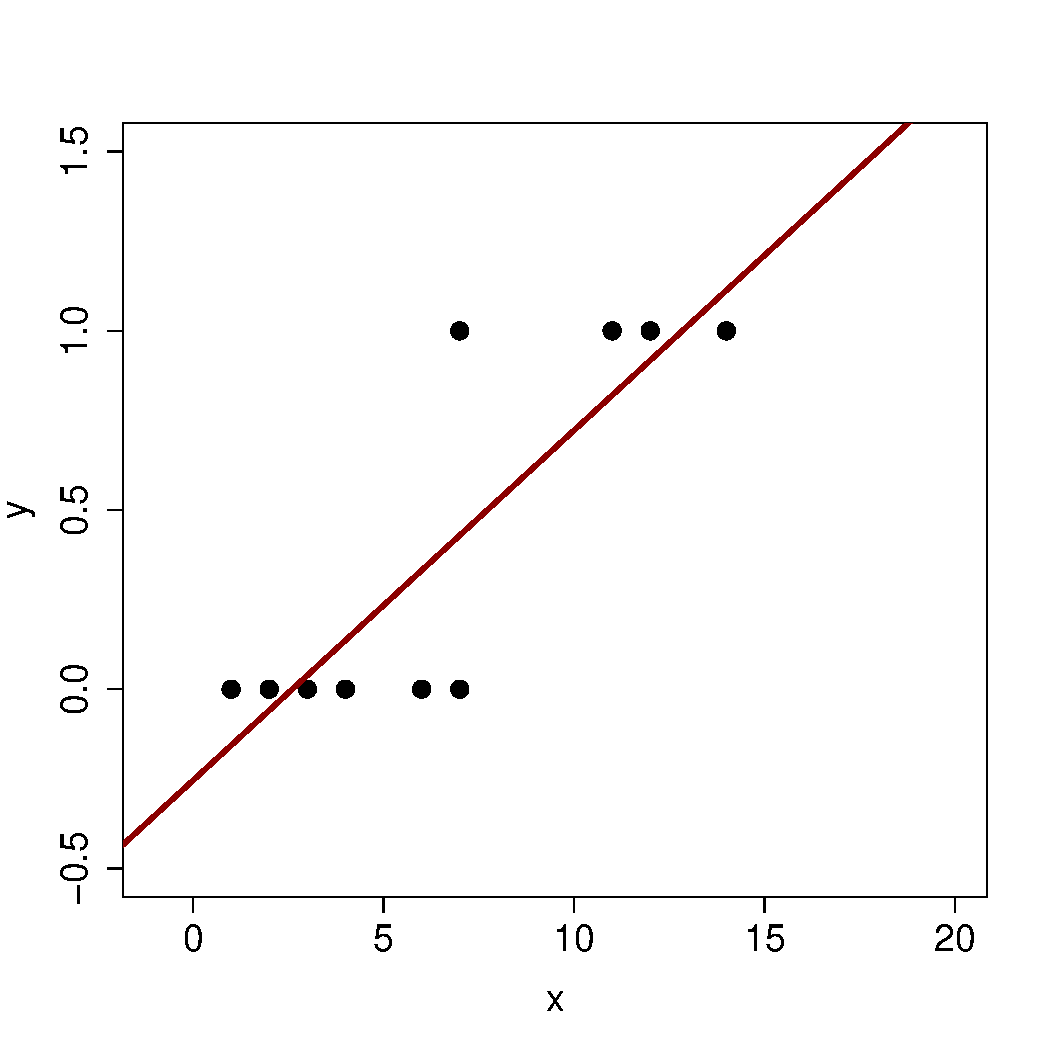
\includegraphics[width=0.4\textwidth]{lm_on_dichotomous}
  \end{center}
\end{frame}

\subsection{GLM Grundlagen}

\begin{frame}
  {Logits}
  \begin{itemize}[<+->]
    \item Vorhersage der \alert{Eintrittswahrscheinlichkeiten}
    \item \alert{lineare Kombination der Regressoren} wie beim LM
    \item Linearkombination ergibt die \alert{Logits} ($z$):
  \end{itemize}
  \pause
  \begin{center}
    $z=\beta_1x_1 + \beta_2x_2 + \cdots + \beta_nx_n + \beta_0$
  \end{center}
\end{frame}

\begin{frame}
  {Link-Funktion}
  Die Logits werden transformiert in Eintrittswahrscheinlichkeiten\\
  mittels der \alert{logistischen Funktion} ($e$ ist die Euler-Konstante):
  \begin{center}
    $\hat{p}(y=1)=\frac{1}{1+e^{-z}}$
  \end{center}
  \pause
  Bei der \alert{binären Vorhersage} dann:
  \begin{center}
    \[\hat{y}=
      \begin{cases}
	0 & \text{wenn }\hat{p}(y=1)\leq0.5 \\
        1 & \text{wenn }\hat{p}(y=1)>0.5 \\
      \end{cases}
    \]
  \end{center}
\end{frame}

\begin{frame}
  {Darstellung des Effekts der Logit-Transformation}
  Die transformierten Logits als $\hat{p}(y=1)$:
  \begin{center}
    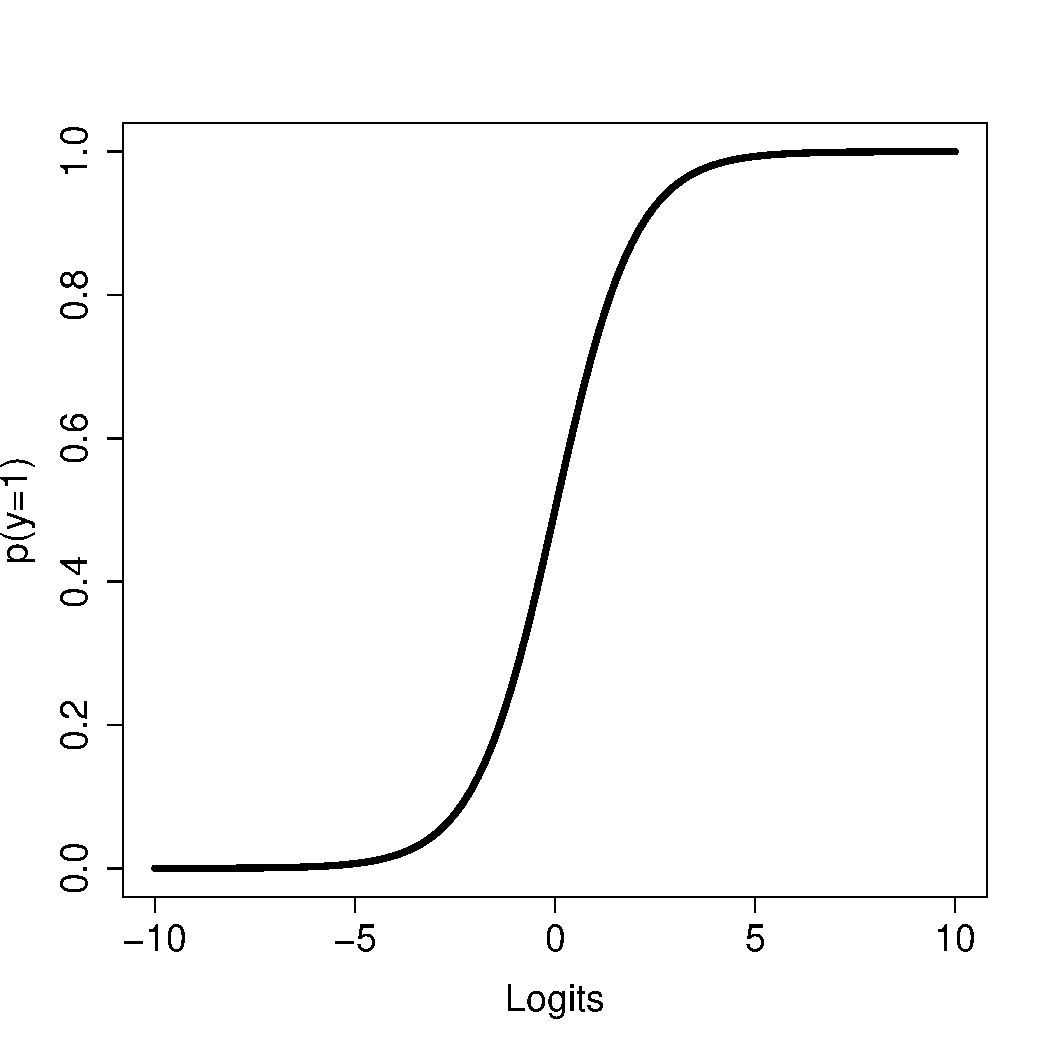
\includegraphics[width=0.4\textwidth]{logits}
  \end{center}
\end{frame}

\begin{frame}
  {Interpretation der Koeffizienten}
  \begin{itemize}[<+->]
    \item Interpretation der Koeffizienten nur \alert{indirekt} möglich
    \item $\beta_i$ positiv $\Rightarrow$ positiver Einfluss auf $\hat{p}(y=1)$
    \item $\beta_i$ negativ $\Rightarrow$ negativer Einfluss auf $\hat{p}(y=1)$
    \item Stärke des Einflusses: \alert{nicht linear}
    \item linearer Einfluss nur auf die Logits, nicht auf $\hat{p}(y=1)$
  \end{itemize}
\end{frame}

\begin{frame}
  {Chancen (Odds) des Modells}
  \begin{itemize}[<+->]
    \item Chance (Odds): $\text{o(y=1)} = \frac{p(y=1)}{1-p(y=1)}$
    \item Die Chancen des Modells verteilen sich (zum Glück) einfach:
  \end{itemize}
  \pause
  \begin{center}
    $\text{o(y=1)} = \frac{p(y=1)}{1-p(y=1)}\alert{=e^z}$\\[3ex]
    Beachte: $ln(e^z)=z=Logits$
  \end{center}
  \pause
  \begin{itemize}[<+->]
    \item Die Chance liegt offensichtlich in $[0, \infty]$.
    \item Mit steigender Wahrscheinlichkeit gehen die Odds gegen $\infty$.
    \item Bei einem Logit von 3 ist die Chance für $y=1$\\
      doppelt so hoch wie bei einem Logit von 1.5 usw.
  \end{itemize}
\end{frame}

\begin{frame}
  {Beziehung zwischen Wahrscheinlichkeit und Odds}
  In der Interpretation stellen die Odds die Linearität her,\\
  die den Wahrscheinlichkeiten bei der log.\ Regression fehlen.
  \begin{center}
    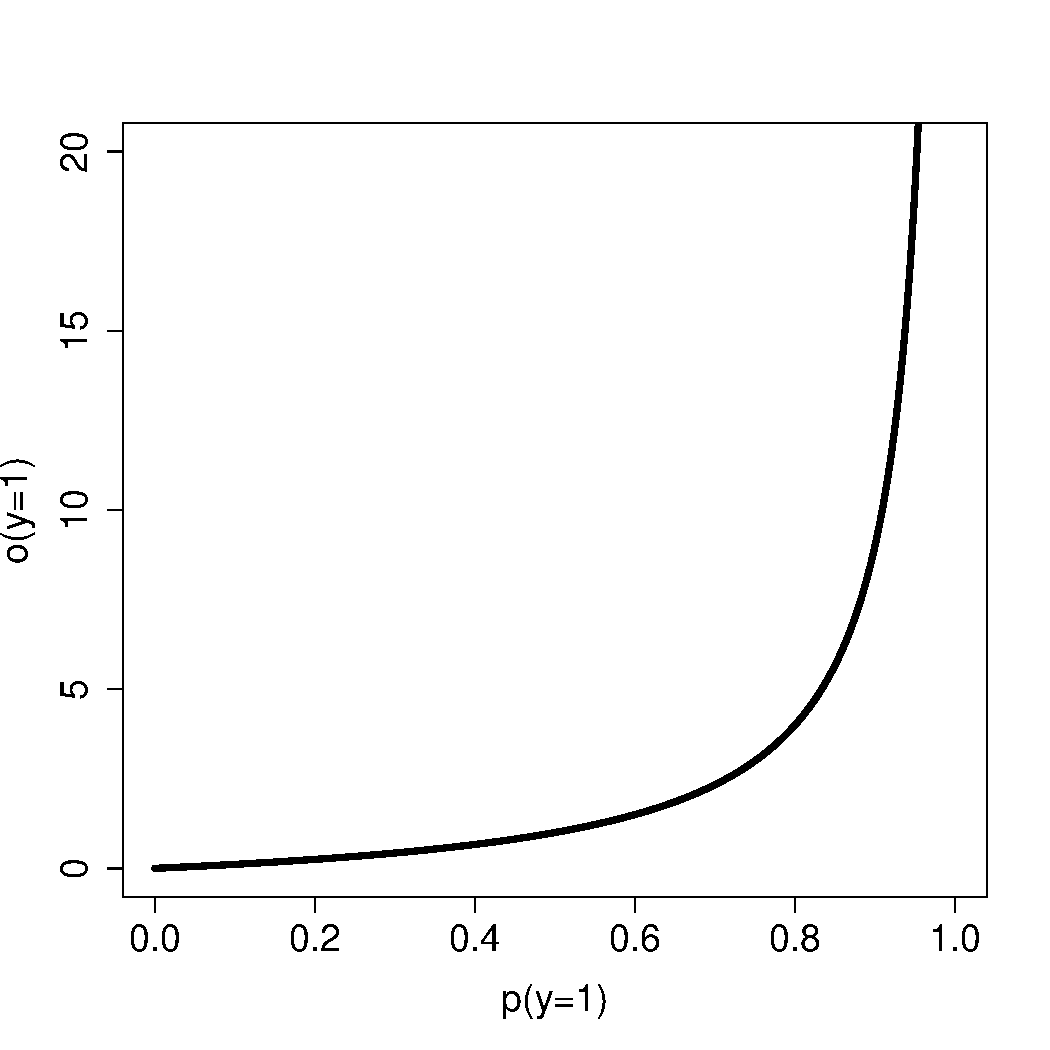
\includegraphics[width=0.4\textwidth]{odds}
  \end{center}
\end{frame}

\begin{frame}
  {Effekt-Koeffizienten}
  Für die Interpretation der einzelnen Koeffizienten $\beta_i$\\
  im Sinne eines Chancenverhältnisses:
  \begin{center}
    \alert{$or(y=1|x_i)=e^{\beta_i}$}
  \end{center}
  \pause
  In Worten: Steigt $x_i$ (intervallskaliert!) um eine Einheit,\\
  dann steigt die Chance für $y=1$ um $e^{\beta_i}$.\\
  \vspace{0.5cm}
  \pause
  Ein Chancenverhältnis von $1$ entspricht einem Koeffizienten $0$,\\
  also einem ohne jeglichen Effekt.
\end{frame}

\begin{frame}
  {Zusammenfassung nach Backhaus et al., S.\ 437}
  Beziehungen zwischen den Maßen\\
  sowie ihre Wertebereiche.\\
  \vspace{0.5cm}
  \begin{center}
    \scalebox{0.9}
    {
      \begin{tabular}[h!]{|c|c||c|c|c|}
	\hline
	\multicolumn{2}{|c||}{\textbf{Einzel-Koeffizient}} & \multicolumn{3}{c|}{\textbf{Gesamtmodell}} \\
	\hline
	\textbf{Koeffizient} & \textbf{Chancenverhältnis} & \textbf{Logit} & \textbf{Chance} & $\mathbf{\hat{p}(y=1)}$ \\
	\hline\hline
	$\beta>0$ & $e^{\beta}>1$ & steigt um $\beta x$ & steigt um $e^{\beta x}$ & steigt \\
	\hline
	$\beta<0$ & $e^{\beta}<1$ & sinkt um $\beta x$ & sinkt um $e^{\beta x}$ & sinkt \\
	\hline\hline
	$[-\infty,+\infty]$ & $[0,+\infty]$ & $[-\infty,+\infty]$ & $[0..+\infty]$ & $[0,1]$ \\
	\hline
      \end{tabular}
    }
  \end{center}
\end{frame}

\subsection{Maximum Likelihood}

\begin{frame}
  {Maximum-Likelihood-Schätzung}
  \begin{itemize}[<+->]
    \item Es gibt keine direkte Lösung für die Koeffizientenberechnung.
    \item Das Schätzverfahren funktioniert iterativ.
    \item Es kommt der sog.\ Maximum-Likelihood-Schätzer zum Einsatz.
  \end{itemize}
\end{frame}

\begin{frame}
  {Maximum Likelihood für Modell I}
  \begin{itemize}[<+->]
    \item Es gibt beliebig viele Modelle = Belegungen für die $\beta$-Koeffizienten
    \item Das \alert{wahrscheinlichste Modell angesichts der Beobachtungen} ist zu finden.
    \item In den Beobachtungsdaten für jeden Fall $k$: \alert{$y_k=1$ oder $y_k=0$}
    \item Für jeden Beobachtungswert $y_k$ betrachtet man:
  \end{itemize}
  \pause
  \begin{center}
    $p_k=(\frac{1}{1+e^{-z_k}})^{y_k}\cdot(1-\frac{1}{1+e^{-z_k}})^{1-y_k}$
  \end{center}
\end{frame}

\begin{frame}
  {Maximum Likelihood für Modell II}
  \begin{center}
    $p_k=(\frac{1}{1+e^{-z_k}})^{y_k}\cdot(1-\frac{1}{1+e^{-z_k}})^{1-y_k}$
  \end{center}
  \begin{itemize}[<+->]
    \item $z_k$ ist der Modell-Logit für die zu $y_k$ empirische gemessenen $x$.
    \item In den $(~)$ steht \alert{links die vom Model geschätzte Wahrscheinlichkeit $\hat{p}(y_k)$}\\
      und \alert{rechts jeweils die Gegenwarscheinlichkeit dazu $1-\hat{p}(y_k)$}.
    \item Wenn der Modellwert nahe an $0$ (\zB $0.1$) und $y_k=0$ ist:\\
      \alert{$p_k=(0.1)^0\cdot(0.9)^1=1\cdot 0.9=0.9$} ("`gute"' Approximation)
    \item Wenn der Modellwert bei gleichen empirischen Daten umgekehrt ist:\\
      \alert{$p_k=(0.9)^0\cdot(0.1)^1=1\cdot 0.1=0.1$} ("`schlechte"' Approximation)
    \item Die $p_k$ messen also die Güte der vom Modell vorhergesagten\\
      Wahrscheinlichkeit für jeden beobachteten Datenpunkt.
  \end{itemize}
\end{frame}

\begin{frame}
  {Maximum Likelihood für Modell III}
  \begin{itemize}[<+->]
    \item Bei unabhängigen Ereignissen $E_{1..n}$ gilt:\\
      $P(E_1+E_2+\cdots+E_n)=\prod\limits_i P(E_i)$
    \item Die Wahrscheinlichkeit eines Modells (seine "`Likelihood"')\\
      angesichts aller empirischen Werte $y_k$ ist also:
  \end{itemize}
  \pause
  \begin{center}
    \alert{$L=\prod\limits_k p_k$}
  \end{center}
  \pause
  \begin{itemize}[<+->]
    \item Der Maximum Likelihood-Schätzer maximiert $L$\\
      für die Belegungen der $\beta$-Koeffizienten (= konkurrierende Modelle).
  \end{itemize}
\end{frame}

\subsection{Nominale Unabhängige}

\begin{frame}
  {Dummy-Kodierung}
  Wie bei der LM-Variante der ANOVA müssen kategoriale Unabhängige\\
  mit mehr als zwei Ausprägungen als dichotome Dummy-Variablen kodiert werden.\\
  \vspace{0.5cm}

  \pause
  \textbf{Beispiel für dreiwertige Variable A und Dummy-Regressoren $x_{1..3}$}

  \begin{center}
    \begin{tabular}[h!]{|c|c|c|c|}
      \cline{2-4}
      \multicolumn{1}{c|}{} & $\mathbf{A=1}$ & $\mathbf{A=2}$ & $\mathbf{A=3}$ \\
      \hline
      $\mathbf{x_1=}$ & $\mathbf{1}$ & $0$ & $0$ \\
      $\mathbf{x_2=}$ & $0$ & $\mathbf{1}$ & $0$ \\
      $\mathbf{x_3=}$ & $0$ & $0$ & $\mathbf{1}$ \\
      \hline
    \end{tabular}
  \end{center}
  \pause
  Achtung! De facto gibt es für einen kategorialen Regressor mit $k$ Ausprägungen\\
  nur $k-1$ Dummies (s.\ Abschnitt zum Intercept).
\end{frame}

\begin{frame}
  {Nominale Unabhängige in Modellgleichungen}
  Beispiel für eine als $x_{1..3}$ dummy-kodierte Unabhängige $A$\\
  und eine intervallskalierte Unabhängige $x_4$:
  \vspace{0.5cm}
  \pause
  \begin{center}
    $\hat{p}(y=1)=\frac{1}{1+e^{-z}}$\\[3ex]
    mit $z=\beta_1x_1+\beta_2x_2+\beta_3x_3+\beta_4x_4+\beta_0$
  \end{center}
  \pause
  \vspace{0.5cm}
  Dabei treten die Werte auf:
  \begin{itemize}[<+->]
    \item $x_{1..3}$: $0$ oder $1$
    \item Wenn $x_1=1$, dann $x_2=0$ und $x_3=0$ usw.
    %\item $x_4\in{\rm I\!R}$
  \end{itemize}
\end{frame}

\begin{frame}
  {Effekt-Koeffizienten für Nominale}
  (Wh.:) Für die Interpretation der einzelnen Koeffizienten $\beta_i$\\
  im Sinne eines Chancenverhältnisses:
  \begin{center}
    \alert{$or(y=1|x_i)=e^{\beta_i}$}
  \end{center}
  \pause
  In Worten \alert{für nominale Regressoren} bzw.\ ihr \alert{dichotomen Dummies}:\\
  \vspace{0.5cm}
  \pause
  Wenn $x_i=1$ ($x_i$ ist dichotom skaliert!),\\
  dann ist die Chance $o(y=1)$ um $e^{\beta_i}$ höher als bei $x_i=0$.\\
  \pause
  Andere Fälle gibt es wegen der dichotomen Skalierung nicht.
\end{frame}

\begin{frame}
  {Der Intercept in GLMs}
  \begin{itemize}[<+->]
    \item "`Intercept"' ($\beta_0$) in GLMs $\neq$ Schnittpunkt mit y-Achse
      \vspace{0.5cm}
    \item \alert{intervallskalierte Regressoren}:
      \begin{itemize}
	\item einfachstes binomiales GLM: \alert{$\hat{p}(y=1)=\beta_1x_1+\mathbf{\beta_0}$}
	\item Wenn $x_1=0$, wird $\beta_0$ vorhergesagt.
      \end{itemize}
      \vspace{0.5cm}
    \item bei \alert{Dummy-Variablen} wird eine zur Referenz-Kategorie:
      \begin{itemize}
	\item GLM mit drei Dummies: \alert{$\hat{p}(y=1)=\beta_{Akk}\cdot x_{Akk}+\beta_{Dat}\cdot x_{Dat}+\mathbf{\beta_{Nom}}$}
	\item "`Alle Regressoren werden 0"' heißt hier, es liegt Nom vor.
	\item Die Dummies modellieren\\
	  den \alert{Unterschied zwischen Referenz (Nom) und den anderen Fällen}.
	\item Die Referenzkategorie sollte die häufigste sein, besonders bei Interaktionen.
      \end{itemize}
  \end{itemize}
\end{frame}

\begin{frame}
  {Interaktionen}
  \begin{itemize}[<+->]
    \item nichts wesentlich anderes als in LM
    \item vereinte Effekte, die über die Einzeleffekte hinausgehen
    \item bei Interpretationsschwierigkeiten ggf.\ nachlesen
  \end{itemize}
\end{frame}

\subsection{Modellselektion}

\begin{frame}
  {Prinzip der Modellauswahl}
  \begin{itemize}[<+->]
    \item Signifikanz wird für das Modell und Koeffizienten bestimmt.
    \item Allerdings: Signifikanz heißt nicht automatisch Modellgüte.
    \item Je "`weniger signifikant"' ein Regressor,\\
      desto wahrscheinlicher kann er ohne Güteverlust entfernt werden.
    \item Modellselektion: Auswahl des \alert{einfachsten Modells}\\
      mit der \alert{größten Modellgüte}.
    \vspace{0.5cm}
    \item Achtung bei dichotomen Dummy-Regressoren:\\
      Immer \alert{alle} Dummies im Modell lassen oder herausnehmen,\\
      die zu einer kategorialen Unabhängigen gehören!
  \end{itemize}
\end{frame}

\begin{frame}
  {Weglassen von Faktoren: Log-Likelihood-Ratio-Test}
  \begin{enumerate}[<+->]
    \item Weglassen des Regressors mit der geringsten Signifikanz
    \item Vergleich des vollen und des reduzierten Modells
    \item bei nicht-signifikantem Unterschied: Regressor weglassen
    \item von vorne beginnen\ldots
  \end{enumerate}
  \pause
  \begin{center}
    Log-Likelihood-Ratio für Likelihood des vollen ($L_f$) und reduzierten ($L_r$) Modells:\\
    \alert{$LR=(-2\cdot ln(L_r)) - (-2\cdot ln(L_f))$}
  \end{center}
  \pause
  \begin{center}
    Test: \alert{Unter der H0 $L_r=L_f$ ist die LR $\chi^2$-verteilt}\\
    mit $df=df_f-df_r$ ($df$ jeweils: Zahl der Regressoren)\\
    \vspace{0.25cm}
    \pause
    Ist die LR \alert{größer} als der kritische Wert: Regressor im Modell lassen!
  \end{center}
\end{frame}

\begin{frame}
  {Weglassen von Faktoren: AIC}
  Regressoren-Selektion auf Basis des \alert{Akaike Information Criterion}:
  \begin{itemize}[<+->]
    \item Ablauf wie bei LR-Test
    \item Maß für Modellvergleich ist das AIC
    \item Informationstheoretisches Maß:\\
      \alert{Distanz des Modells zur (geschätzten) absoluten Realität}
    \item Je kleiner das AIC, desto besser das Modell.
    \item Achtung: Nur zum Vergleich \alert{eingebetteter Modelle} verwenden,\\
      also bei gleichem Datensatz, und wenn das reduzierte Modell\\
      eine Teilmenge der Regressoren des vollen enthält.
  \end{itemize}
\end{frame}

\subsection{Modellevaluation}

\begin{frame}
  {Evaluation der Koeffizienten}
  \begin{itemize}[<+->]
    \item Signifikanzbestimmung für einzelne Regressoren
    \item wie bei LM: \alert{Standardfehler} für jeden Regressor
    \item darauf basierend: \alert{z-Wert} für jeden Regressor\ldots
    \item und \alert{z-Test} auf Basis der Normalverteilung
  \end{itemize}
\end{frame}

\begin{frame}
  {Log-Likelihood-Ratio-Test für Modelle}
  \begin{itemize}[<+->]
    \item Log-Likelihood-Ratio-Test für Gesamtheit aller Regressoren
    \item volles Modell (ggf.\ nach Eliminierung von Koeffizienten)
    \item \alert{Nullmodell}, das nur einen konstanten Term zur Vorhersage nutzt
    \item ähnlich den Modellvergleichen im Kapitel "`ANOVA als LM"'
  \end{itemize}
\end{frame}

\begin{frame}
  {Pseudo-$R^2$}
  \begin{itemize}
    \item auch Vergleich des vollen Modells und Nullmodels
    \item Interpretation wie gewohnt: \alert{Varianzerklärung}
  \end{itemize}
  \pause
  \begin{center}
    Cox \& Snell: $R^2_{C}=1-(\frac{L_0}{L_f})^{\frac{2}{n}}$
  \end{center}
  \pause
  Problem: \alert{Geht nicht bis 1!}
  \pause
  \begin{center}
    \alert{Nagelkerke: $R^2_N=\frac{R^2_{C}}{R^2_{max}}$}\\[2ex]
    mit $R^2_{max}=1-(L_0)^{\frac{2}{n}}$
  \end{center}
\end{frame}

\begin{frame}
  {Vorhersagegüte}
  \begin{itemize}[<+->]
    \item gutes GLM $\Rightarrow$ gute Vorhersagen
    \item einfache Vorhersagegüte: \alert{Anteil der richtigen Vorhersagen}
    \item instruktiv: \alert{Vergleich mit "`Baseline"'}\\
      (= Anteil der richtigen Vorhersagen bei Vorhersage der modalen Kategorie)
      \vspace{0.5cm}
    \item Problem wie bei Fehlerreduktion:\\
      \alert{auch bei starkem Effekt nicht unbedingt Umkehrung der modalen Kategorie}
  \end{itemize}
\end{frame}

\begin{frame}
  {Überdispersion}
  \begin{itemize}[<+->]
    \item zugrundegelegte Verteilung: \alert{Binomialverteilung}
    \item Überdispersion: Varianz ist größer als für Binomialverteilung angenommen
    \item mögliche Gründe:
      \begin{itemize}[<+->]
	\item unbeobachtete Heterogenität (fehlende erklärende Variablen)
	\item Gruppenbildung (= Beobachtungen nicht unabhängig)
      \end{itemize}
    \end{itemize}
    \pause
    \begin{center}
      Schätzung des \alert{Dispersionsparameters}:\\[3ex]
      \alert{$\hat{\phi}=\sum (\frac{R_P}{df_R})^2$}\\[3ex]
      wobei: \alert{$R_P$ ist das Pearson-Redidual} (hier nicht behandelt) und\\[2ex]
      $df_R$ die \alert{Residual-Freiheitsgrade $n-p$}, $p$ die Anzahl der Modellparameter
    \end{center}
\end{frame}

\begin{frame}
  {Lösung bei Überdispersion}
  \begin{itemize}[<+->]
    \item Problem: \alert{$\hat{\phi}$ deutlich über $1$}
    \item Lösung: Schätzung der Parameter bleibt (im Ergebnis) gleich
    \item aber für die Evaluation der Koeffizienten:
      \begin{itemize}[<+->]
	\item Signifikanzschätzung mit größeren Standardfehlern
	\item t-Verteilung statt Normalverteilung (z-Werte)
      \end{itemize}
     \vspace{0.5cm}
    \item Ein "`Quasi-Likelihood-Modell"' folgt im Wesentlichen dieser Strategie.
  \end{itemize}
\end{frame}

\begin{frame}
  {(Multi-)kollinearität}
  \begin{itemize}[<+->]
    \item \alert{(Multi-)kollinearität}: Abhängigkeit zwischen Regressoren
    \item Probleme: $\beta$-Fehler, Überanpassung, ungenaue Koeffizientenschätzung
    \item Test: \alert{Varianzinflations-Faktoren} (nicht im Detail behandelt)
    \item Lösungen z.\,B.: mehr Daten, Regressoren wegglassen
    \item Test des Modells auf Robustheit trotz Kollinearität (z.\,B.\ Kreuzvalidierung)
  \end{itemize}
\end{frame}

\begin{frame}
  {Varianzhomogenität}
  Die Residuen werden im GLM zwar anders berechnet,\\
  sind aber trotzdem ein Maß für die Varianz.\\[3ex]
  \alert{Die Varianz sollte nicht mit den Regressorausprägungen variieren!}\\

  \begin{center}
    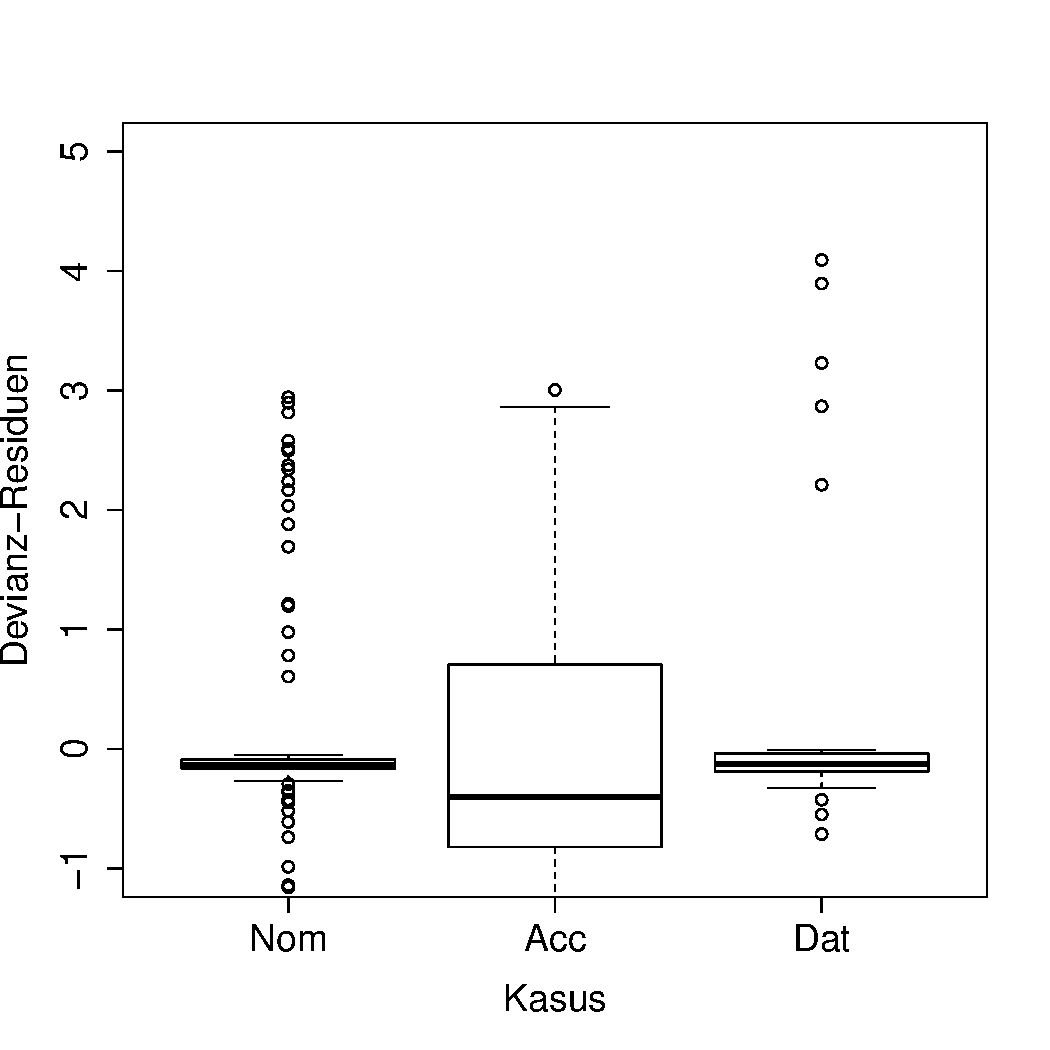
\includegraphics[width=0.4\textwidth]{glmvarianz}
  \end{center}
\end{frame}

\subsection{Alternativen und Lösungen}

\begin{frame}
  {Kreuzvalidierung}
  \begin{itemize}[<+->]
    \item bei Problemen: Test auf \alert{Robustheit des Modells}
    \item Idee bei $k$-facher Kreuzvalidierung:
      \begin{enumerate}
	\item teile Daten in $k$ Teile
	\item Modellanpassung auf $k-1$ von $k$ Teilen
	\item Prüfung der Vorhersage auf verbleibendem Teil
	\item Modell ist Robust, wenn die Parameter in der Kreuzvalidierung\\
	  nicht wesentlich anders geschätzt werden als im Ursprungsmodell
      \end{enumerate}
    \item wenn $k=n$: \alert{Leave-One-Out-Kreuzvalidierung}
    \item verwandtes Verfahren: \alert{Bootstrapping} (mit Zurücklegen)
  \end{itemize}
\end{frame}

\begin{frame}
  {Andere GLMs}
  Einige typische Anwendungsfälle für nicht-binomiale GLMs:\\

  \begin{itemize}[<+->]
    \item Zähldaten: \alert{Poisson}
    \item Zähldaten mit Überdispersion: \alert{negativ-binomial}
    \item bestimmte Intervalldaten in $[0,\infty]$: \alert{Gamma}
    \item viele Nullen: \alert{zero-inflated} Varianten
  \end{itemize}
  \pause
  \begin{center}
    Das Vademecum, vor allem für \texttt{R}-Benutzer:\\
    \cite{ZuurEa2009}
  \end{center}
\end{frame}

\begin{frame}
  {Gemischte Modelle (GLMMs)}
  \begin{itemize}[<+->]
    \item typisches gemischtes Modell: \alert{mit Zufallseffekten}
    \item Idee: Varianzunterschiede oder Dispersion durch \alert{Gruppen}
    \item mögliche Gruppen in linguistischen Experimenten:
      \begin{itemize}
	\item Werte von einem Probanden bei Befragung, Rating-Studie
	\item Werte zu einem Lexem bei Korpusstudie
	\item Werte aus einer Textsorte bei Korpusstudie
      \end{itemize}
    \item ideal: Gruppeneffekte durch zusätzliche normale Regressoren auflösen
    \item sonst (vereinfacht): \alert{Schätzung eines Intercepts pro Gruppe}
    \item Typisch für Zufallseffekte: In der GG sind vermutlich viel mehr Ausprägungen\\
      vorhanden, als gemessen (wie \zB Sprecher oder Lexeme) wurden.
  \end{itemize}
\end{frame}

\begin{frame}
  {Generalisierte Additive Modelle (GAMs)}
    GAMs oder \alert{"`nichtparametrische Regression"'}
    \begin{center}
      $\hat{y}=f_1(x_1)+f_2(x_2)+\cdots+f_n(x_n)+\beta_0$
    \end{center}
    \begin{itemize}[<+->]
      \item $f_n$: besondere Art von \alert{Funktion}, die geschätzt wird
      \item Wenn die Funktionen ungefähr linear sind, ist ein GLM genauso gut.
      \item Interpretation von GAMs: viel schwieriger als GLMs
      \item letzter Ausweg bei schlechtem GLM
    \end{itemize}
\end{frame}

\subsection{In \texttt{R}}

\begin{frame}[allowframebreaks]
  {In \texttt{R}}
  \small
  \begin{enumerate}[<+->]
    \item Modell-Anpassung:\\
      \texttt{> m <- glm(y~x1+x2*y3, data=mydata, family="binomial")}\\
      \texttt{> summary(m)}
    \item Chancenverhältnisse für Koeffizienten:\\
      \texttt{> exp(coef(m))}
    \item 95\%-Konfidenzintervalle für Chancenverhältnisse:\\
      \texttt{> exp(confint(m))}
    \item Log-Likelihood extrahieren:\\
      \texttt{> logLik(m)}
    \item Nagelkerke $R^2$:\\
      \texttt{> library(fmsb); NagelkerkeR2(m)}
    \item LR-Test:\\
      \texttt{> m0 <- glm(y~1, data=mydata, family="binomial")}\\
      \texttt{> lr <- (-2*logLik(m0))-(-2*logLik(m))}\\
      \texttt{> pchisq(lr, m\$rank-m0\$rank)}
    \item Modellselektion (wenn nicht von Hand):\\
      \texttt{> drop1(m)}
    \item Varianzinflationsfaktoren:\\
      \texttt{> library(car); vif(m)}
    \item Dispersion $\hat{\phi}$ schätzen:\\
      \texttt{> sum(resid(m, type="pear")\^{}2 / df.residual(m))}
    \item Vorhersagegüte:\\
      \texttt{> pred <- ifelse(predict(m) <= 0.5, 0, 1)}\\
      \texttt{> tab  <- table(pred, mydata\$response)}\\
      \texttt{> sum(diag(tab))/sum(tab)}
    \item Fehlerrate in Kreuzzvalidierung (hier $k=10$):\\
      \texttt{library(boot); cv.glm(mydata, m, K=10)\$delta}
  \end{enumerate}
\end{frame}
